\documentclass[tikz]{standalone}
\usepackage{tikz,amsmath}
\usetikzlibrary{positioning} 
\begin{document}
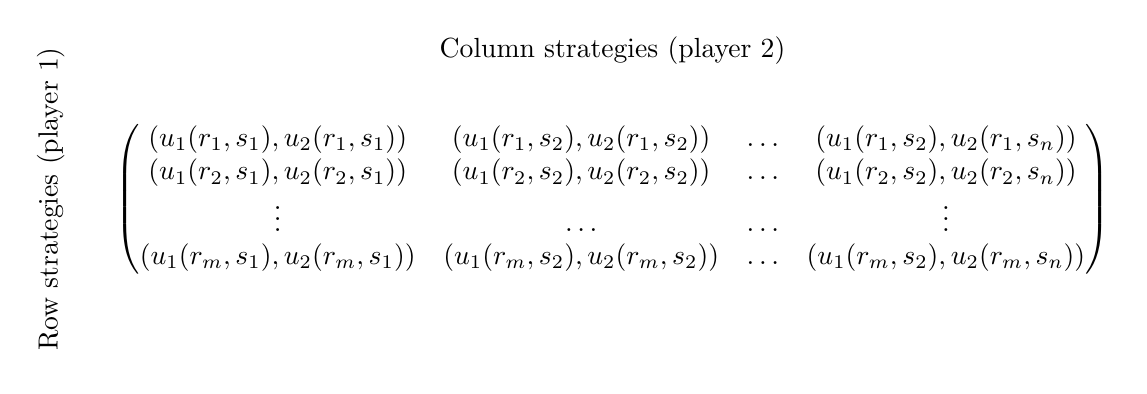
\begin{tikzpicture}[grow=right, sloped]
    \node (bimatrix) {$\begin{pmatrix}
(u_1(r_1,s_1),u_2(r_1,s_1))&(u_1(r_1,s_2),u_2(r_1,s_2))&\dots&(u_1(r_1,s_2),u_2(r_1,s_n))\\
(u_1(r_2,s_1),u_2(r_2,s_1))&(u_1(r_2,s_2),u_2(r_2,s_2))&\dots&(u_1(r_2,s_2),u_2(r_2,s_n))\\
\vdots&\dots&\dots&\vdots\\
(u_1(r_m,s_1),u_2(r_m,s_1))&(u_1(r_m,s_2),u_2(r_m,s_2))&\dots&(u_1(r_m,s_2),u_2(r_m,s_n))\\
\end{pmatrix}$};
    \node [above=.5cm of bimatrix] {Column strategies (player 2)};
    \node [left=1cm of bimatrix, rotate=90, anchor=north, text width= 4cm, text centered] {Row strategies (player 1)};
\end{tikzpicture}
\end{document}
